\documentclass[12pt]{article}
\usepackage[pdftex]{graphicx}
% \usepackage[numbers]{natbib}
\usepackage{natbib}
\usepackage{color}
\usepackage{amsmath}
\usepackage{amssymb}
\usepackage{verbatim}
\usepackage{mathpazo}
\usepackage{setspace}
\usepackage{multirow}
\usepackage{fullpage}
\usepackage{lscape}
\usepackage{array}
\usepackage{paralist}
\usepackage{fancyhdr}
\usepackage{graphicx}
\usepackage{makecell}
\usepackage{longtable}
\usepackage{xr}
\usepackage{subfig}
\externaldocument{ms}
\bibliographystyle{gcb}
\parindent=2em
\setlength{\parskip}{1ex}

\RequirePackage{lineno}

\begin{document}

\doublespacing
\linenumbers

%% reset counters for the SI \clearpage
\renewcommand{\thesection}{S\arabic{section}} \setcounter{section}{0}
\renewcommand{\theequation}{S\arabic{equation}}
\setcounter{equation}{0} \renewcommand{\thetable}{S\arabic{table}}
\setcounter{table}{0} % reset counter
\renewcommand{\thefigure}{S\arabic{figure}} \setcounter{figure}{0}
\setcounter{page}{1}

\newcommand{\lkmcomment}[1] {
  \textcolor{red}{\it{[#1]}}
}

% \begin{center} {\LARGE\textbf{Supplementary Information}}
% \end{center}

\begin{table}
  \renewcommand*\arraystretch{1.25}
  \centering
  \caption{Number of samples per year at each assembling hedgerow site. Asterisks indicate
    the year of planting for each restoration site. Sampling was not
    conducted in 2010 because resources were allocated to other
    projects.} 
  \begin{tabular}{lllllllllll}
    \hline
    \multicolumn{10}{c}{\hspace{10em}Year}\\
    & Site & 2006 & 2007 & 2008 & 2009 & 2010 & 2011 & 2012 & 2013 & 2014\\
    \hline
    % \multirow{5}{*}{\thead{Assembling \\ Hedgerows}}
    &Barger & 2 & 3 & 3* & 3 & - & 3 & 4 & 5 & 3 \\
    &Butler & 4 & 3* & 3 & 3 & - & 3 & 4 & 5 & 3 \\ 
    &Hrdy & - & 3 & 3* & 3 & - & 3 & 4 & 5 & 3 \\
    &MullerB & 2 & 3* & 3 & 3 & - & 3 & 4 & 5 & 3 \\
    &Sperandio & - & 3 & 3* & 3 & - & 3 & 4 & 5 & 3 \\
    \hline
  \end{tabular}
  \label{tab:maturing}
\end{table}
\clearpage

\begin{table}
  \renewcommand*\arraystretch{1.25}
  \centering
  \caption{Number of samples per year at each non-assembling hedgerow
    site. Asterisks indicate the site was sampled five or more times
    and thus included in the change point analysis.} 
  \begin{tabular}{lllllllllll}
    \hline
    \multicolumn{10}{c}{\hspace{10em}Year}\\
    & Site & 2006 & 2007 & 2008 & 2009 & 2010 & 2011 & 2012 & 2013 & 2014\\
    \hline
    % \multirow{19}{*}{\thead{Non-assembling \\ Hedgerows}}
    &Anderson & - & - & - & - & 4 & - & - & - & - \\
    &Berm & - & - & - & - & - & - & 3 & 5 & 3\\
    &Bobcat & 4 & - & - & - & - & - & - & - & -\\
    &CLBL & 4 & - & 1 & - & - & - & - & - & -\\
    &CR1-1 & - & - & - & - & - & - & 3 & 5 & 3\\
    &CR29 & - & - & - & - & - & - & 4 & 5 & 3\\
    &Fong* & - & - & 1 & 4 & 4 & 2 & 4 & 5 & 3\\
    &FongWest & - & - & - & - & - & - & 4 & 5 & 3\\
    &Gilmer & - & - & - & - & - & - & 4 & 4 & 2 \\
    &Harlan* & - & - & - & 3 & - & 2 & 4 & 5 & 3\\
    &Johnston & - & - & - & - & - & - & - & 5 & 3 \\
    &Martinez & - & - & - & - & - & - & 4 & 5 & 3\\
    &MullerM* & - & - & - & - & 4 & 2 & 6 & 5 & 3\\
    &Oakdale & - & - & - & - & - & - & 4 & 5 & -\\
    &PutahCreek & - & - & - & - & - & - & 4 & 5 & 3\\
    &RLong & - & - & - & - & - & - & 4 & 5 & 3 \\
    &Rominger* & - & - & - & 4 & 4 & 2 & 4 & 5 & 3\\
    &Tractor* & - & - & - & 4 & - & 1 & 4 & 5 & 3\\
    &Voelz & - & - & - & - & - & - & 4 & - & -\\
    \hline
  \end{tabular}
  \label{tab:mature}
\end{table}
\clearpage

\begin{table}
  \renewcommand*\arraystretch{1.25}
  \centering
  \caption{Number of samples per year at each non-assembling field
    margin site. Asterisks indicate the site was sampled five or more times
    and thus included in the change point analysis.} 
  \begin{tabular}{lllllllllll}
    \hline
    \multicolumn{10}{c}{\hspace{10em}Year}\\
    & Site & 2006 & 2007 & 2008 & 2009 & 2010 & 2011 & 2012 & 2013 & 2014\\
    \hline
    % \multirow{29}{*}{\thead{Non-assembling \\ field margins}}
    &Barn* & - & - & - & 3 & 4 & - & 3 & 5 & 3\\
    &BC1 & 4 & 3 & 3 & - & - & - & - & - & -\\
    &BC2* & - & 3 & 3 & 3 & - & 3 & 4 & 4 & 3\\
    &Best & - & - & - & - & - & - & 3 & 4 & 2\\
    &Chamberlain* & - & 3 & 3 & 3 & - & 2 & 4 & 4 & 2\\
    &CircleG & - & - & - & 4 & - & - & 4 & 5 & 3\\
    &CR1-1Control & - & - & - & - & - & - & 1 & 5 & 2\\
    &DQU* & 4 & 3 & 3 & 3 & - & 3 & 4 & 5 & 3\\
    &GC1 & 4 & - & - & - & - & - & - & - & -\\
    &Gnoss & 4 & - & - & - & - & - & - & - & -\\
    &Gregory* & - & 3 & 3 & 3 & - & 3 & 4 & 5 & 3\\
    &H16* & 4 & 3 & 3 & 3 & - & 3 & 3 & 5 & 3\\
    &Hatanaka & - & - & - & 4 & - & - & 3 & 3 & 1\\
    &Hays & - & - & - & - & - & - & 3 & - & -\\
    &HC1 & - & 3 & 3 & 3 & - & 3 & - & - & -\\
    &Joe* & - & - & - & 4 & 4 & - & 3 & 5 & 1\\
    &Joost & - & - & - & - & 4 & - & - & - & -\\
    &Loop & - & - & - & - & - & - & - & 5 & 3\\
    &Maria & - & - & - & - & - & - & - & 5 & 3\\
    &Mariani & - & - & - & - & - & - & 3 & - & -\\
    &MC1* & - & 3 & 3 & 3 & - & 3 & 4 & 3 & 1\\
    &Rock & 4 & - & - & - & - & - & - & - & -\\
    &Roosevelt & - & - & - & - & - & - & - & 1 & -\\
    &RSlough & - & - & - & - & - & - & 3 & 5 & 3\\
    &Spiva* & - & 3 & 3 & 3 & - & 3 & 2 & 4 & 2\\
    &Turkovich* & 4 & 3 & 3 & 3 & - & 3 & 4 & 5 & 3\\
    &USS* & 4 & 3 & 3 & 3 & - & 3 & 4 & 4 & 2\\
    &YoloAirport & - & - & - & - & - & - & 4 & 5 & 2\\
    &Zamora & - & - & - & - & 4 & - & 5 & 4 & 3\\
    \hline
  \end{tabular}
  \label{tab:controls}
\end{table}
\clearpage


\begin{figure}
  \centering
  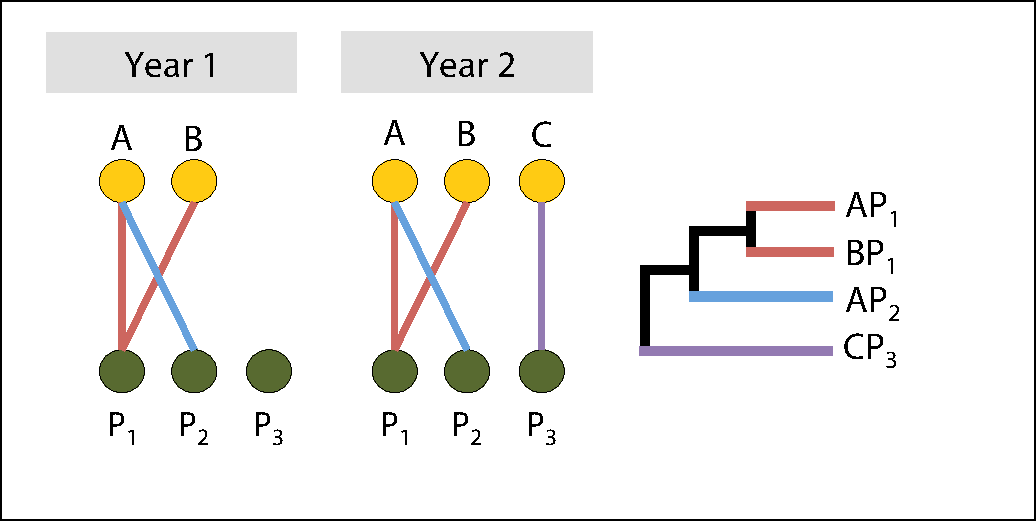
\includegraphics[width=.8\textwidth]{figures/scheme.pdf}
  \caption{Diagram illustrating the analysis to examine the temporal
    turnover of interactions weighted based on their similarity (after
    Ahn et al. 2010). A, B and C are animal species, and Ps are plant
    species. The dendrogram depicts the interaction similarity across
    years based on the number of shared constituent species.}
  \label{fig:methods}
\end{figure}
\clearpage



\begin{figure}
  \centering
  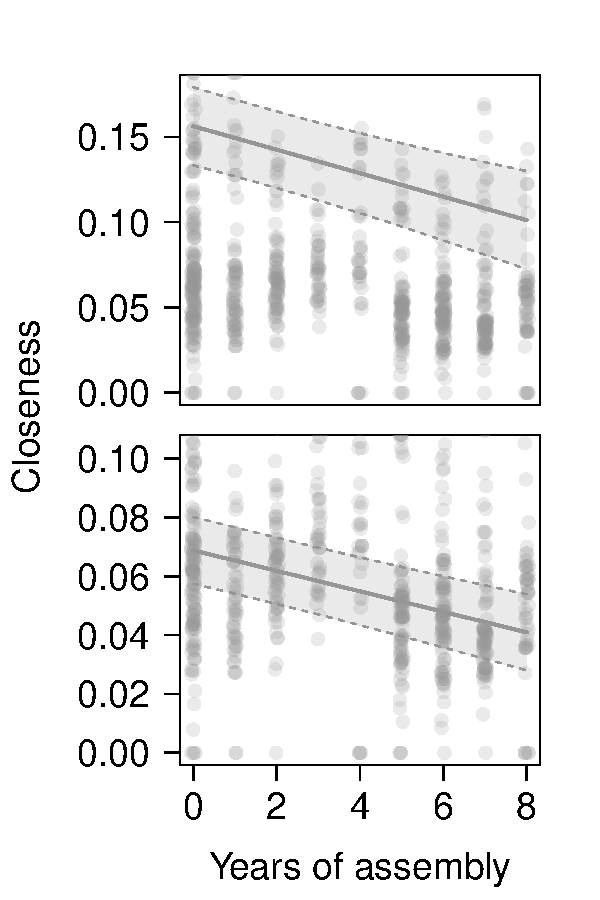
\includegraphics[width=.6\textwidth]{../analysis/speciesLevel/figures/closenessPanel.pdf}
  \caption{The closeness of pollinators and plants decreased slightly
    through time. Points represent means for each species across
    sites. The solid line indicates the mean slope estimate and the
    dashed lines are the $95\%$ confidence intervals around the
    estimate.}
  \label{fig:closeness}
\end{figure}
\clearpage

\begin{figure}[!tbp]
  \centering
  \subfloat[Before]{\includegraphics[width=0.4\textwidth]{figures/before.pdf}\label{fig:f1}}
%  \hfill
  \subfloat[After]{\includegraphics[width=0.4\textwidth]{figures/after.pdf}\label{fig:f2}}
  \caption{The before and after hedgerows were planted, at the same location.}
\end{figure}
\clearpage


\end{document}

%%% Local Variables:
%%% mode: latex
%%% TeX-PDF-mode: t
%%% End:
